\documentclass[conference]{IEEEtran}
\IEEEoverridecommandlockouts

\usepackage{cite}
\usepackage{amsmath,amssymb}
\usepackage{graphicx}
\usepackage{booktabs}
\usepackage{url}
\usepackage{xcolor}

\begin{document}

\title{Predicting Latent Toxoplasmosis: A Machine Learning Approach Integrating Demographic, Behavioral, and Health Questionnaires}

\author{
\IEEEauthorblockN{Vickelsteins August Santoso}
\IEEEauthorblockA{\textit{Department} \\
\textit{University}\\
City, Country \\
email}
\and
\IEEEauthorblockN{Timothy Jonathan Imannuel}
\IEEEauthorblockA{\textit{Department} \\
\textit{University}\\
City, Country \\
email}
}

\maketitle

% =====================================================================
\begin{abstract}
\textit{Toxoplasma gondii} infection is common and usually silent, and it can only be confirmed with a blood test. This study asks how well routine survey answers can identify adults who carry \textit{T.~gondii} IgG antibodies. We used 5,006 adults from the U.S. National Health and Nutrition Examination Survey (NHANES) 2013--2014, of whom 750 (15.0\%) were seropositive. Logistic regression, random forest, gradient boosting and XGBoost were compared on four nested feature sets: demographics; plus a \textit{Toxocara} antibody marker; plus behaviour and mental health; and plus lifestyle features taken from an earlier questionnaire study of people with HIV. Models were compared with repeated cross-validation and a corrected $t$-test, and the final model was evaluated once on a held-out test set. No feature group beyond demographics and no complex model gave a meaningful gain, so the final model was logistic regression on demographics alone, which needs no blood test. On the test set it reached a ROC-AUC of 0.700 (95\% CI 0.654--0.747) and a PR-AUC of 0.316 against a prevalence of 0.150, and its predicted risks were well calibrated (slope 0.90). Birthplace and years in the U.S., age and race/ethnicity drove the predictions. Survey data can rank adults by infection risk, but only modestly, and the lifestyle features from the HIV study did not carry over to the general population.
\end{abstract}

\begin{IEEEkeywords}
\textit{Toxoplasma gondii}, NHANES, machine learning, logistic regression, calibration, seroprevalence
\end{IEEEkeywords}

% =====================================================================
\section{Introduction}

\textit{Toxoplasma gondii} is a parasite that infects warm-blooded animals, including humans. People are usually infected by eating undercooked meat, by contact with soil or water contaminated with cat feces, or by eating contaminated produce. After the first infection the parasite stays in the body for life, and most people have no symptoms. A recent meta-analysis of 320 studies estimated that about 31\% of people worldwide have been exposed \cite{sengupta2025}. In the United States, the NHANES 2009--2010 survey found an age-adjusted seroprevalence of 12.4\%, with the highest rates among older adults, people born outside the U.S. and people with lower socioeconomic status \cite{jones2014}.

Latent infection is not always harmless. Seropositive people have reported worse health on many self-reported measures, although the effects were small \cite{flegr2016}. A recent NHANES study of older adults linked infection to lower scores on one cognitive test \cite{kruszon2023}, while another found no link with depression \cite{gale2021}. These consequences are still uncertain, which makes cheap ways to estimate infection risk useful for research.

Infection can only be confirmed with a laboratory test, usually a blood test for IgG antibodies. Such tests are costly and need trained staff, which limits testing in large surveys and in communities with few health resources \cite{achtziger2025}. Questionnaire data, in contrast, is cheap and already collected in many surveys. Ichwan \textit{et al.} \cite{ichwan} recently used machine learning (ML) on questionnaire answers from Indonesian people living with HIV and reported a weighted F1-score of 0.80 in one subgroup. That study was small (78 people after filtering), and it is unknown whether its features help in the general population.

This study asks five research questions:
\begin{itemize}
\item \textbf{RQ1}: How well can survey data predict \textit{T.~gondii} seropositivity in U.S. adults, compared with a dummy baseline and an age-only baseline?
\item \textbf{RQ2}: Which groups of variables improve prediction beyond demographics: a \textit{Toxocara} antibody marker, behaviour and mental health variables, or the lifestyle features used in \cite{ichwan}?
\item \textbf{RQ3}: Which model (logistic regression, random forest, gradient boosting or XGBoost) performs best, and is the difference meaningful?
\item \textbf{RQ4}: Which factors are independently associated with infection, and which drive the final model's predictions?
\item \textbf{RQ5}: Are the final model's predicted risks well calibrated on unseen data?
\end{itemize}

% =====================================================================
\section{Related Work}

\textit{Epidemiology.} Studies using NHANES serology consistently find that age, birth outside the U.S. and lower socioeconomic status predict seropositivity \cite{jones2014}, and infection is still more common among U.S. adults living in poverty \cite{cuffey2021}. These studies describe risk factors. They do not test how accurately the factors predict who is infected, or whether predicted risks are well calibrated.

\textit{Health, mood and cognition.} Flegr and Escudero \cite{flegr2016} studied 1,486 volunteers and found that the 333 seropositive participants reported worse health on 28 of 29 health variables, although the effect sizes were small and the design cannot show cause. Kruszon-Moran \textit{et al.} \cite{kruszon2023} studied 2,643 NHANES adults aged 60 and over. Infection was linked to lower scores on three cognitive tests, but after adjustment the link remained for only one of them. Gale \textit{et al.} \cite{gale2021} found no association with depression in 2,484 NHANES 2013--2014 adults and 2,271 UK Biobank participants. These mixed results suggest that no single health questionnaire is a strong predictor on its own.

\textit{Low-cost detection without a blood test.} Achtziger \textit{et al.} \cite{achtziger2025} classified latent infection from response times in a short computer task. In 79 RhD-negative participants (12 seropositive), the method had a sensitivity of 91.7\% and a specificity of 97.0\%. However, it works only for RhD-negative people, was validated in a small, young sample, and needs a purpose-built task.

\textit{Questionnaire-based machine learning.} Ichwan \textit{et al.} \cite{ichwan} predicted seropositivity from questionnaire answers covering diet, sexual behaviour, drug use, hygiene, oral health and economic status. Of 186 people with HIV, 78 remained after filtering. The data were balanced with SMOTE and reduced with PCA, and five models were compared on one 70/30 split, so the test set had 24 people. The best model reached a weighted F1-score of 0.80 in the subgroup with higher economic scores and lower dietary risk, and 0.45--0.54 in the opposite subgroup. Probabilities and calibration were not reported.

\textit{Machine learning on NHANES.} Comparing several models on NHANES data and explaining the best one with SHAP \cite{lundberg2017} is an established approach, for example for vitamin D deficiency from nine interview variables \cite{guo2024}. In that study, logistic regression and gradient boosting reached validation AUCs of 0.77--0.79, while XGBoost reached 1.0. The near-perfect result is unusual for simple interview variables, so we use that study as a methodological template rather than a benchmark. We found no comparable ML study for \textit{T.~gondii} serostatus.

% =====================================================================
\section{Materials and Methods}

\subsection{Data Source}
NHANES is a cross-sectional survey of the U.S. population that combines home interviews, a health examination and laboratory tests \cite{johnson2014}. We used the 2013--2014 cycle and merged public files on the participant ID (SEQN).

\subsection{Study Population and Outcome}
We included all adults aged 18 years or older with a \textit{T.~gondii} IgG result, giving 5,006 participants. A participant was classed as positive if their IgG level was 33~IU/mL or higher. Following CDC instructions, borderline results (27--33~IU/mL) were retested and coded as negative \cite{cdc_sstoxo}; this applied to 11 people. In total, 750 participants (15.0\%) were positive.

\subsection{Variables and Data Cleaning}
Eight files provided demographics (age, sex, race/ethnicity, years living in the U.S., education and family income-to-poverty ratio) \cite{cdc_demo}, health and behaviour (self-rated health, sleep hours, reported sleep trouble, smoking, alcohol use and the PHQ-9 depression score \cite{kroenke2001}) and a \textit{Toxocara} antibody test \cite{cdc_sstoca}. \textit{Toxocara} eggs are shed in dog and cat feces and contaminate soil \cite{healy2022}, and antibodies to the two parasites often occur together \cite{liu2018}, so we used \textit{Toxocara} as a marker of soil exposure.

To answer the last part of RQ2, five more files were added: sexual behaviour, drug use, the oral health examination, the oral health questionnaire and the HIV antibody test. From these we built features that match the questions in \cite{ichwan} as closely as NHANES allows (Table~\ref{tab:paper}). Some questions were asked only in certain age groups; for example, nobody over 69 was asked about sexual behaviour or drug use, so these values were left missing. When a question was skipped because it did not apply, such as condom use for someone with no partner in the past year, the value was set to zero. One feature almost exactly repeated another and was left out, and lifetime partner counts were log-transformed.

``Refused'' and ``Don't know'' answers were treated as missing. Smoking status, drinks per drinking day and the PHQ-9 total were derived from the raw items, and adults aged 18--19, who answer a different education question, were mapped onto the adult scale.

\begin{table}[t]
\caption{Features Matching the Questionnaire of Ichwan \textit{et al.} \cite{ichwan}}
\label{tab:paper}
\centering
\small
\begin{tabular}{p{0.38\columnwidth}p{0.52\columnwidth}}
\toprule
Column in \cite{ichwan} & NHANES 2013--2014 feature \\
\midrule
Condom use during oral sex & Protection when performing oral sex \\
Partner's condom use & Frequency of sex without a condom \\
Frequency of anal intercourse & Ever had anal sex; sex frequency in past year \\
Sexual risk score & Lifetime partners, same-sex partner, age at first sex, STD history \\
Injection drug use, used needles & Ever injected drugs \\
Other risk (drug use) & Ever used cocaine, heroin or methamphetamine \\
Tooth loss & Missing teeth (dental examination) \\
Natural tooth loss & Teeth loosened without injury \\
Mouth ulcers & Aching in the mouth, past year \\
HIV status (study population) & HIV antibody test \\
\bottomrule
\end{tabular}
\end{table}

\subsection{Feature Sets}
Four nested feature sets were defined, each adding to the last:
\begin{itemize}
\item \textbf{Set A}: demographics.
\item \textbf{Set B}: Set A plus \textit{Toxocara} serostatus.
\item \textbf{Set C}: Set B plus self-rated health, sleep hours, sleep trouble, smoking status, drinks per day and PHQ-9 score.
\item \textbf{Set D}: Set C plus the features in Table~\ref{tab:paper}.
\end{itemize}
Survey design variables (weights, strata, PSU) and the participant ID were never used as features.

\subsection{Preprocessing}
All analysis was done in Python with pandas \cite{mckinney2010}, scikit-learn \cite{pedregosa2011} and XGBoost \cite{chen2016}. All preprocessing was learned inside each training fold, so no information leaked from the data used for testing. Categorical features were filled with the most common value and one-hot encoded. Numeric features were filled with the median and standardised. Features with many missing values, including all Set D features, also received a binary ``was missing'' indicator.

\subsection{Models}
We compared logistic regression (L2 penalty, $C=1$), random forest \cite{breiman2001} (500 trees, minimum leaf size 10), histogram gradient boosting \cite{friedman2001} (learning rate 0.05, depth 3, 300 iterations) and XGBoost \cite{chen2016} (300 trees, learning rate 0.05, depth 3, row and column subsampling 0.8). Two baselines were used: a dummy model that gives everyone the training prevalence, and logistic regression on age alone. No class weighting or oversampling was used, so the models output risk probabilities.

\subsection{Validation Design and Metrics}
The data were split once into a stratified 80\% training set (4,004 people) and a 20\% test set (1,002 people). All model comparison used the training set only, with 5-fold stratified cross-validation repeated three times (15 folds); every model used the same folds. The main metric was ROC-AUC. We also report PR-AUC, which is more informative when positives are uncommon \cite{saito2015}, and the Brier score, which measures the accuracy of the predicted probabilities. Accuracy was not used because it is misleading at a 15\% positive rate.

\subsection{Statistical Comparison}
Fold scores share training data, so a standard paired $t$-test underestimates variance. We used the corrected resampled $t$-test \cite{nadeau2003}:
\begin{equation}
t = \frac{\bar{d}}{\sqrt{\left(\frac{1}{k} + \frac{n_{\text{test}}}{n_{\text{train}}}\right)\hat{\sigma}_d^2}},
\end{equation}
where $\bar{d}$ and $\hat{\sigma}_d^2$ are the mean and variance of the per-fold ROC-AUC differences, $k=15$, and $n_{\text{test}}/n_{\text{train}} = 0.25$. A difference counted as meaningful only if ROC-AUC improved by at least 0.01 \emph{and} $p<0.05$. If a feature group or a more complex model did not meet this rule, the simpler option was kept.

\subsection{Final Model and Test-Set Evaluation}
The penalty strength $C$ of the final model was tuned on the training folds with the same rule. A risk cut-off was chosen on out-of-fold training predictions by maximising Youden's index. The final model was then fitted on the whole training set and evaluated once on the test set. We report bootstrap 95\% confidence intervals (2,000 resamples), a calibration slope and plot, and sensitivity, specificity and predictive values at the cut-off. A decision curve compares the net benefit of testing people chosen by the model with testing everyone or no one, where the net benefit at risk threshold $p_t$ is
\begin{equation}
\text{NB} = \frac{TP}{n} - \frac{FP}{n}\cdot\frac{p_t}{1-p_t}.
\end{equation}
Adjusted odds ratios (ORs) with 95\% confidence intervals came from an unpenalised logistic regression with all Set C variables on the training set. SHAP values \cite{lundberg2017} on the test set showed which features drive the final model.

% =====================================================================
\section{Results}

\subsection{Cohort Characteristics}
Table~\ref{tab:cohort} shows seropositivity by group. Positivity rose with age and was higher among foreign-born adults, Other Hispanic adults, those with less education and those who were \textit{Toxocara}-positive. The mean age was 48.0 years (SD 18.4).

\begin{table}[t]
\caption{Seropositivity by Group (NHANES 2013--2014 Adults, $n=5{,}006$)}
\label{tab:cohort}
\centering
\small
\begin{tabular}{lrr}
\toprule
Group & $n$ & Positive (\%) \\
\midrule
\textbf{Overall} & 5006 & 15.0 \\
\midrule
Age 18--39 & 1819 & 8.7 \\
Age 40--59 & 1629 & 15.3 \\
Age 60--80 & 1558 & 22.0 \\
\midrule
Female & 2630 & 13.6 \\
Male & 2376 & 16.5 \\
\midrule
U.S.-born & 3627 & 11.6 \\
Foreign-born, $<$10 y in U.S. & 251 & 26.3 \\
Foreign-born, 10--19 y & 371 & 21.3 \\
Foreign-born, $\geq$20 y & 690 & 24.1 \\
Foreign-born, unknown & 66 & 27.3 \\
\midrule
Mexican American & 713 & 15.4 \\
Other Hispanic & 450 & 30.4 \\
Non-Hispanic White & 2238 & 13.4 \\
Non-Hispanic Black & 913 & 14.2 \\
Non-Hispanic Asian & 537 & 10.4 \\
Other / multiracial & 155 & 11.0 \\
\midrule
Less than 9th grade & 381 & 29.1 \\
9th--11th grade & 737 & 19.3 \\
High school / GED & 1150 & 17.0 \\
Some college & 1533 & 11.4 \\
College graduate+ & 1201 & 10.5 \\
\midrule
\textit{Toxocara} positive & 337 & 34.1 \\
\textit{Toxocara} negative & 4669 & 13.6 \\
\bottomrule
\end{tabular}
\end{table}

\subsection{Model Comparison (RQ1--RQ3)}
Table~\ref{tab:cv} gives the cross-validated ROC-AUC on the training set. All four models clearly beat both baselines (RQ1): the dummy model had a ROC-AUC of 0.500 and the age-only model 0.632, while the models reached 0.694--0.724. Logistic regression on Set B did best (ROC-AUC 0.724, PR-AUC 0.337, Brier 0.116).

Adding \textit{Toxocara} raised ROC-AUC by 0.004--0.006 for every model, which was consistent but below the 0.01 rule. Behaviour and mental health changed ROC-AUC by $-0.007$ to $+0.003$, and the features from \cite{ichwan} by $-0.012$ to $-0.001$ (RQ2). No tree-based model beat logistic regression on any set; the differences ranged from $-0.016$ to $-0.001$ (RQ3). None of these differences met the rule, so the final model was logistic regression on Set A, which needs no blood test.

\begin{table}[t]
\caption{Cross-Validated ROC-AUC on the Training Set (Mean of 15 Folds)}
\label{tab:cv}
\centering
\small
\begin{tabular}{lcccc}
\toprule
Model & Set A & Set B & Set C & Set D \\
\midrule
Logistic regression & 0.720 & \textbf{0.724} & 0.719 & 0.714 \\
Random forest & 0.710 & 0.716 & 0.718 & 0.717 \\
Gradient boosting & 0.707 & 0.711 & 0.704 & 0.694 \\
XGBoost & 0.710 & 0.714 & 0.712 & 0.700 \\
\midrule
\multicolumn{5}{l}{Baselines: dummy 0.500; age-only logistic regression 0.632} \\
\bottomrule
\end{tabular}
\end{table}

\subsection{Final Model on the Test Set (RQ5)}
Tuning $C$ gave no gain, so the default ($C=1$) was kept. On the test set, the final model reached a ROC-AUC of 0.700 (Table~\ref{tab:test}), slightly below the cross-validated 0.720 but within the confidence interval. It ranked people better than age alone by 0.059 (95\% CI 0.018--0.103).

\begin{table}[t]
\caption{Test-Set Results ($n=1{,}002$, 150 Positive; 95\% Bootstrap CI)}
\label{tab:test}
\centering
\small
\begin{tabular}{lccc}
\toprule
Model & ROC-AUC & PR-AUC & Brier \\
\midrule
Dummy & 0.500 & 0.150 & 0.127 \\
Age-only LR & 0.641 & 0.216 & 0.124 \\
 & (0.593--0.689) & (0.175--0.266) & \\
Final model & \textbf{0.700} & \textbf{0.316} & \textbf{0.118} \\
 & (0.654--0.747) & (0.253--0.393) & \\
\bottomrule
\end{tabular}
\end{table}

The predicted risks matched the observed rates well (Fig.~\ref{fig:calib}). The average predicted risk was 14.9\%, and 15.0\% of the test set was positive. The calibration slope was 0.90 (ideal 1), so the highest predicted risks were slightly too high.

\begin{figure}[t]
\centering
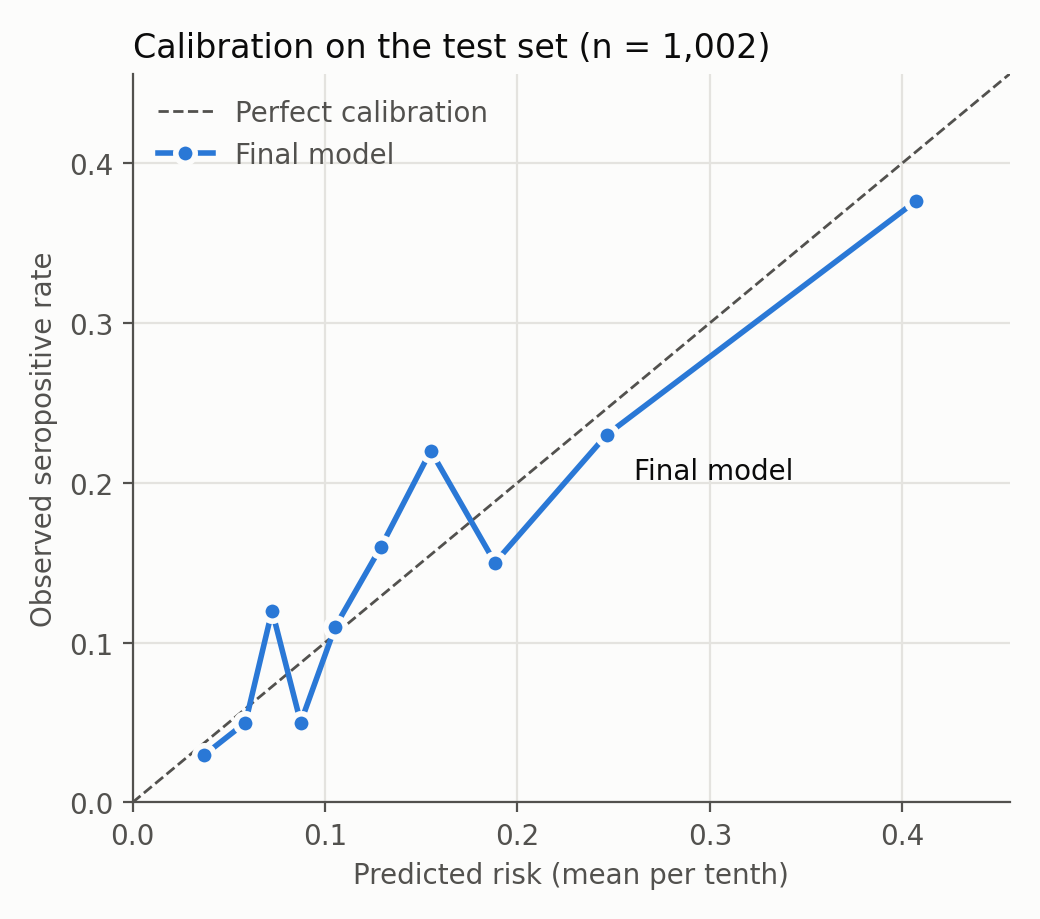
\includegraphics[width=\columnwidth]{calibration_final.png}
\caption{Calibration on the test set: mean predicted risk against the observed rate in each tenth of predicted risk.}
\label{fig:calib}
\end{figure}

At the risk cut-off of 12.4\%, chosen on the training data, the model flagged 47\% of the test set and found 73\% of the positive people (sensitivity 0.73, specificity 0.57). Only 23\% of flagged people were positive, but 92\% of those not flagged were negative. The decision curve (Fig.~\ref{fig:dca}) shows that choosing whom to test with the model beats testing everyone or no one for risk thresholds between 10\% and 40\%, but the gain is small.

\begin{figure}[t]
\centering
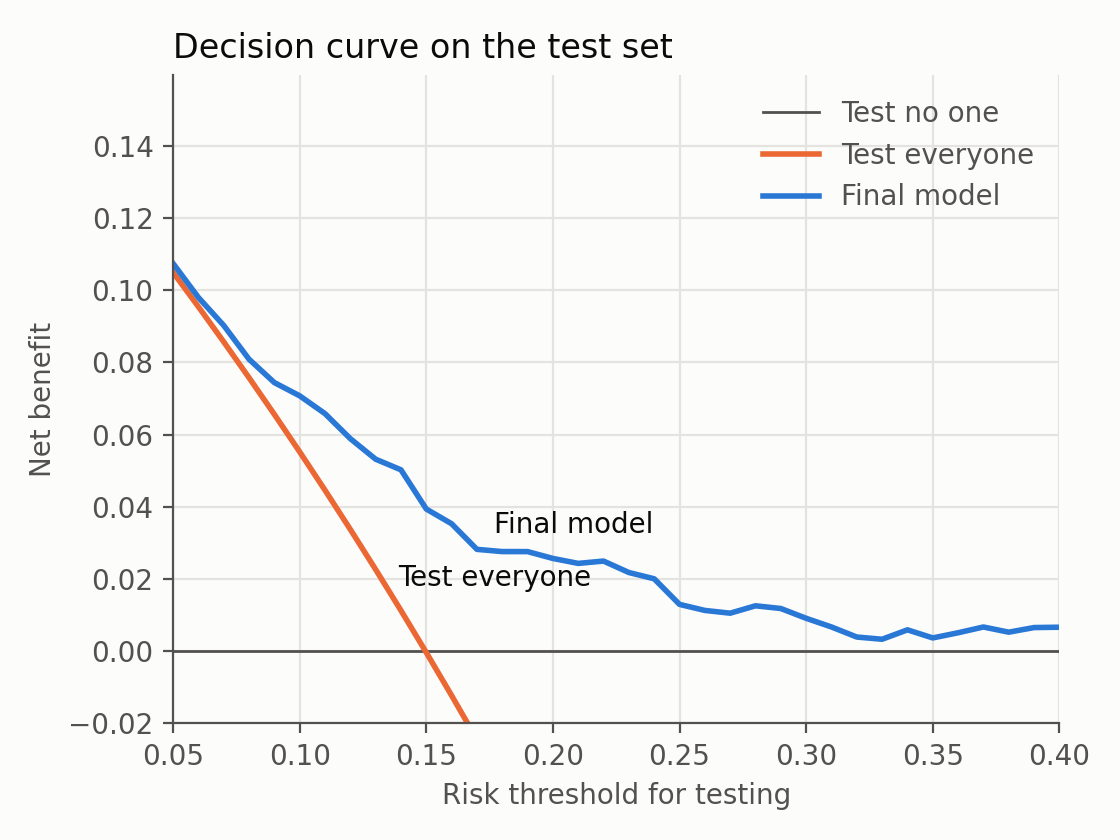
\includegraphics[width=\columnwidth]{decision_curve_final.png}
\caption{Decision curve on the test set.}
\label{fig:dca}
\end{figure}

\subsection{Risk Factors and Model Explanation (RQ4)}
Table~\ref{tab:or} shows the adjusted odds ratios. Infection was more likely with older age, male sex, Other Hispanic ethnicity, birth outside the U.S. and \textit{Toxocara} antibodies. Among foreign-born adults, the odds were highest for recent arrivals and fell with years in the U.S. Infection was less likely with more education and among Mexican American and Non-Hispanic Asian adults. Income, self-rated health, sleep, smoking, alcohol and PHQ-9 score were not significant.

\begin{table}[t]
\caption{Adjusted Odds Ratios (Training Set, $n=4{,}004$)}
\label{tab:or}
\centering
\small
\begin{tabular}{lc}
\toprule
Factor & OR (95\% CI) \\
\midrule
Age, per 10 years & 1.34 (1.26--1.43) \\
Male (vs female) & 1.26 (1.04--1.54) \\
Other Hispanic (vs NH White) & 1.55 (1.09--2.20) \\
Mexican American (vs NH White) & 0.64 (0.45--0.91) \\
NH Asian (vs NH White) & 0.34 (0.22--0.52) \\
Foreign-born, $<$10 y in U.S. (vs U.S.-born) & 6.13 (3.95--9.49) \\
Foreign-born, 10--19 y & 3.26 (2.24--4.76) \\
Foreign-born, $\geq$20 y & 2.54 (1.88--3.44) \\
Foreign-born, years unknown & 2.28 (1.09--4.78) \\
Education, per level (1--5) & 0.85 (0.78--0.93) \\
Income-to-poverty ratio, per unit & 0.95 (0.88--1.02) \\
\textit{Toxocara} positive & 1.91 (1.42--2.57) \\
PHQ-9 score, per 5 points & 0.91 (0.80--1.02) \\
\bottomrule
\multicolumn{2}{p{0.9\columnwidth}}{\footnotesize The model also included NH Black and other/multiracial ethnicity, self-rated health, sleep hours, sleep trouble, smoking and alcohol; none was significant. NH = Non-Hispanic.} \\
\end{tabular}
\end{table}

SHAP values (Fig.~\ref{fig:shap}) show that birthplace and years in the U.S. mattered most in the final model, followed closely by age and then race/ethnicity. Income mattered least.

\begin{figure}[t]
\centering
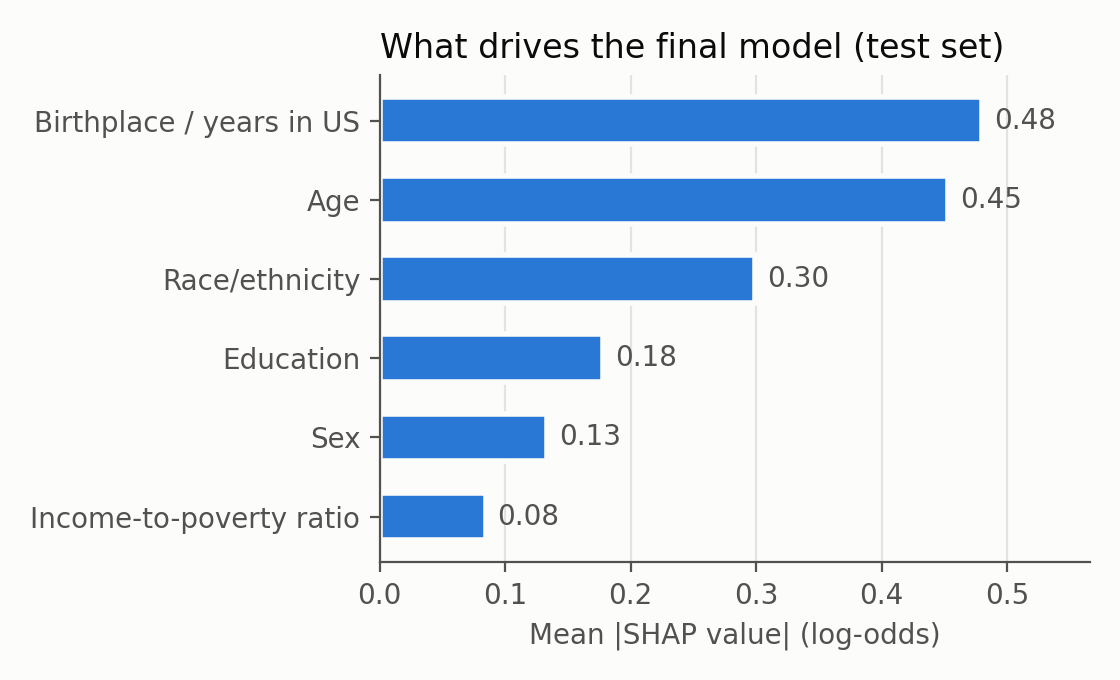
\includegraphics[width=\columnwidth]{shap_final.png}
\caption{Mean absolute SHAP value per feature in the final model on the test set (log-odds scale).}
\label{fig:shap}
\end{figure}

% =====================================================================
\section{Discussion}

Survey data predicted \textit{T.~gondii} seropositivity better than chance and better than age alone, but only modestly. Almost all of the signal came from demographics: birthplace and time in the U.S., age, race/ethnicity and education. This matches the known risk factors \cite{jones2014} and suggests that these variables stand for differences in past exposure, such as food, water and soil in the country of birth, rather than for the people themselves. Logistic regression did as well as the tree-based models, which suggests that the relationships are mostly simple and additive.

The lifestyle features from Ichwan \textit{et al.} \cite{ichwan} added nothing in this population. Their study was done in people living with HIV, where sexual behaviour and drug use may mark risk. In the general U.S. population, infection comes mostly from food, soil and water, which these questions do not measure. Only 18 HIV-positive and 87 injection-drug-using people were in our data, so these features barely varied. The NHANES questions are also not identical to theirs; for example, mouth aching is not the same as mouth ulcers. Our result therefore does not show that their features are useless, only that they do not carry over to the general U.S. population.

\textit{Toxocara} antibodies were clearly linked to infection (OR 1.91) but barely improved prediction. This is not a contradiction: only about 7\% of people were \textit{Toxocara}-positive, so the marker changes the predicted risk for few people. A strong association does not guarantee better prediction. Leaving it out also means the final model needs no blood test at all.

The test ROC-AUC of 0.70 is in the same range as other prediction tools for a laboratory outcome. For vitamin D deficiency, earlier tools reached AUCs of 0.64--0.74, and logistic regression and gradient boosting on nine interview variables reached 0.77--0.79 \cite{guo2024}. In practice, the model's positive predictive value was low (23\%) while its negative predictive value was high (92\%). It is therefore best used to rank people for testing in surveillance or research studies, not as a screening test for individuals.

\subsection{Limitations}
First, the design is cross-sectional and uses one NHANES cycle, so the results show associations, not causes, and the model was not validated on an external dataset. Second, survey weights were not used, so the results describe this sample (15.0\% positive) rather than the whole U.S. population. Third, most predictors are self-reported. Fourth, the features matching \cite{ichwan} are approximations, and several were asked only in certain age groups. Finally, the 2013--2014 data predate current exposure patterns, and NHANES has no questions on cat contact, gardening or eating undercooked meat, which are direct transmission routes.

% =====================================================================
\section{Conclusion}
In 5,006 U.S. adults, a logistic regression on six demographic variables predicted \textit{T.~gondii} seropositivity with a test ROC-AUC of 0.70 and well-calibrated risks. \textit{Toxocara} antibodies, behaviour and mental health variables, lifestyle features from an earlier HIV study, and more complex models gave no meaningful gain. Survey answers can help rank people for serological testing, but better prediction will likely need direct measures of exposure, such as diet and contact with cats and soil. Future work should validate the model on other NHANES cycles and on populations outside the U.S.

% =====================================================================
\section*{Ethics Statement}
NHANES protocols were approved by the NCHS Research Ethics Review Board, and all participants gave written informed consent \cite{cdc_erb}. The \textit{T.~gondii} tests were run on stored samples from participants who agreed to future research use \cite{cdc_sstoxo}. This study used only de-identified public files, in which ages above 80 are recorded as 80 and locations are not released \cite{cdc_demo}. Sexual behaviour and drug use answers were collected privately on a computer in NHANES examination centres. No attempt was made to identify participants, and only grouped results are reported. The model is a research tool, not a diagnostic test, and must not be used for insurance, employment or immigration decisions.

% =====================================================================
\begin{thebibliography}{00}

\bibitem{sengupta2025} P.~P. Sengupta, S.~S. Jacob, K.~P. Suresh, S. Rajamani, and S.~M. Maharana, ``Exploring global trends in human toxoplasmosis seroprevalence by meta-analysis,'' \textit{Exp. Parasitol.}, vol.~275, Art.~no.~108971, 2025, doi: 10.1016/j.exppara.2025.108971.

\bibitem{jones2014} J.~L. Jones, D.~Kruszon-Moran, H.~N. Rivera, C.~Price, and P.~P. Wilkins, ``\textit{Toxoplasma gondii} seroprevalence in the United States 2009--2010 and comparison with the past two decades,'' \textit{Am. J. Trop. Med. Hyg.}, vol.~90, no.~6, pp.~1135--1139, 2014, doi: 10.4269/ajtmh.14-0013.

\bibitem{flegr2016} J.~Flegr and D.~Q. Escudero, ``Impaired health status and increased incidence of diseases in \textit{Toxoplasma}-seropositive subjects -- an explorative cross-sectional study,'' \textit{Parasitology}, vol.~143, no.~14, pp.~1974--1989, 2016, doi: 10.1017/S0031182016001785.

\bibitem{kruszon2023} D.~Kruszon-Moran, D.~Brody, and B.~Pearce, ``Association of infection with \textit{Toxoplasma gondii} and \textit{Toxocara} on cognitive function among US adults aged 60 and over, NHANES 2011--2014,'' \textit{J. Epidemiol. Community Health}, vol.~77, no.~5, pp.~315--321, 2023, doi: 10.1136/jech-2022-219772.

\bibitem{gale2021} S.~D. Gale, L.~D. Erickson, B.~L. Brown, and D.~W. Hedges, ``Examining the relationship between \textit{Toxoplasma gondii} and seropositivity and serointensity and depression in adults from the United Kingdom and the United States: A cross-sectional study,'' \textit{Pathogens}, vol.~10, no.~9, Art.~no.~1101, 2021, doi: 10.3390/pathogens10091101.

\bibitem{achtziger2025} A.~Achtziger, C.~Al\'{o}s-Ferrer, and M.~Garagnani, ``An inexpensive method to measure latent toxoplasmosis and its behavioral consequences,'' \textit{Acta Psychol.}, vol.~254, Art.~no.~104814, 2025, doi: 10.1016/j.actpsy.2025.104814.

\bibitem{ichwan} W.~W. Ichwan, P.~A. Tandra, N.~N. Qomariyah, R.~F. Meirawan, and F.~Setiawan, ``Machine learning-based prediction of seropositive \textit{Toxoplasma gondii} from lifestyle factors,'' \textcolor{red}{[venue and year to be added]}.

\bibitem{cuffey2021} J.~Cuffey, C.~A. Lepczyk, S.~Zhao, and N.~M. Fountain-Jones, ``Cross-sectional association of \textit{Toxoplasma gondii} exposure with BMI and diet in US adults,'' \textit{PLoS Negl. Trop. Dis.}, vol.~15, no.~10, Art.~no.~e0009825, 2021, doi: 10.1371/journal.pntd.0009825.

\bibitem{lundberg2017} S.~M. Lundberg and S.-I. Lee, ``A unified approach to interpreting model predictions,'' in \textit{Proc. Adv. Neural Inf. Process. Syst. (NeurIPS)}, vol.~30, 2017.

\bibitem{guo2024} J.~Guo, Q.~He, and Y.~Li, ``Machine learning-based prediction of vitamin D deficiency: NHANES 2001--2018,'' \textit{Front. Endocrinol.}, vol.~15, Art.~no.~1327058, 2024, doi: 10.3389/fendo.2024.1327058.

\bibitem{johnson2014} C.~L. Johnson, S.~M. Dohrmann, V.~L. Burt, and L.~K. Mohadjer, ``National Health and Nutrition Examination Survey: Sample design, 2011--2014,'' Nat. Center Health Statist., Hyattsville, MD, USA, Vital Health Stat. Ser.~2, no.~162, 2014. [Online]. Available: \url{https://stacks.cdc.gov/view/cdc/22155}

\bibitem{cdc_sstoxo} Centers for Disease Control and Prevention, National Center for Health Statistics, ``National Health and Nutrition Examination Survey 2013--2014 data documentation: \textit{Toxoplasma gondii} antibodies (SSTOXO\_H).'' [Online]. Available: \url{https://wwwn.cdc.gov/Nchs/Data/Nhanes/Public/2013/DataFiles/SSTOXO_H.htm} (accessed Oct.~19, 2026).

\bibitem{cdc_demo} Centers for Disease Control and Prevention, National Center for Health Statistics, ``National Health and Nutrition Examination Survey 2013--2014 data documentation: Demographic variables and sample weights (DEMO\_H).'' [Online]. Available: \url{https://wwwn.cdc.gov/Nchs/Data/Nhanes/Public/2013/DataFiles/DEMO_H.htm} (accessed Oct.~19, 2026).

\bibitem{kroenke2001} K.~Kroenke, R.~L. Spitzer, and J.~B.~W. Williams, ``The PHQ-9: Validity of a brief depression severity measure,'' \textit{J. Gen. Intern. Med.}, vol.~16, no.~9, pp.~606--613, 2001, doi: 10.1046/j.1525-1497.2001.016009606.x.

\bibitem{cdc_sstoca} Centers for Disease Control and Prevention, National Center for Health Statistics, ``National Health and Nutrition Examination Survey 2013--2014 data documentation: Toxocara antibodies (SSTOCA\_H).'' [Online]. Available: \url{https://wwwn.cdc.gov/Nchs/Data/Nhanes/Public/2013/DataFiles/SSTOCA_H.htm} (accessed Oct.~19, 2026).

\bibitem{healy2022} S.~R. Healy, E.~R. Morgan, J.~M. Prada, and M.~Betson, ``Brain food: rethinking food-borne toxocariasis,'' \textit{Parasitology}, vol.~149, no.~1, pp.~1--9, 2022, doi: 10.1017/S0031182021001591.

\bibitem{liu2018} E.~W. Liu, E.~S. Elder, H.~N. Rivera, D.~Kruszon-Moran, S.~Handali, and J.~L. Jones, ``Concurrent seroprevalence of antibodies to \textit{Toxoplasma gondii} and \textit{Toxocara} species in the United States, 2011--2014,'' \textit{Clin. Infect. Dis.}, 2018, doi: 10.1093/cid/ciy729.

\bibitem{mckinney2010} W.~McKinney, ``Data structures for statistical computing in Python,'' in \textit{Proc. 9th Python Sci. Conf.}, 2010, pp.~56--61, doi: 10.25080/Majora-92bf1922-00a.

\bibitem{pedregosa2011} F.~Pedregosa \textit{et al.}, ``Scikit-learn: Machine learning in Python,'' \textit{J. Mach. Learn. Res.}, vol.~12, pp.~2825--2830, 2011.

\bibitem{chen2016} T.~Chen and C.~Guestrin, ``XGBoost: A scalable tree boosting system,'' in \textit{Proc. 22nd ACM SIGKDD Int. Conf. Knowl. Discovery Data Mining}, 2016, pp.~785--794, doi: 10.1145/2939672.2939785.

\bibitem{breiman2001} L.~Breiman, ``Random forests,'' \textit{Mach. Learn.}, vol.~45, no.~1, pp.~5--32, 2001, doi: 10.1023/A:1010933404324.

\bibitem{friedman2001} J.~H. Friedman, ``Greedy function approximation: A gradient boosting machine,'' \textit{Ann. Statist.}, vol.~29, no.~5, pp.~1189--1232, 2001, doi: 10.1214/aos/1013203451.

\bibitem{saito2015} T.~Saito and M.~Rehmsmeier, ``The precision-recall plot is more informative than the ROC plot when evaluating binary classifiers on imbalanced datasets,'' \textit{PLoS ONE}, vol.~10, no.~3, Art.~no.~e0118432, 2015, doi: 10.1371/journal.pone.0118432.

\bibitem{nadeau2003} C.~Nadeau and Y.~Bengio, ``Inference for the generalization error,'' \textit{Mach. Learn.}, vol.~52, pp.~239--281, 2003, doi: 10.1023/A:1024068626366.

\bibitem{cdc_erb} Centers for Disease Control and Prevention, National Center for Health Statistics, ``Ethics Review Board approval.'' [Online]. Available: \url{https://www.cdc.gov/nchs/nhanes/about/erb.html} (accessed Oct.~19, 2026).

\end{thebibliography}

\end{document}
